Im Zuge dieser Diplomarbeit wurden folgende Software-Teile programmiert:
\begin{itemize}
    \item Oberfläche der Applikation (PiBell/MainPage.xaml)
    \item Klassen zur Verwaltung der Dienste (PiBell/Classes/MediaClasses.cs)
    \item Berechtigungsmanagement (PiBell.Android/MainActivity.cs)
    \item Audio-Aufnahme-Service in Android (PiBell.Android/AudioRecordingService.cs)
    \item Audio-Aufnahme-Service in iOS (PiBell.iOS/AudioRecordingService.cs)
\end{itemize}

\begin{figure}[H]
    \centering
    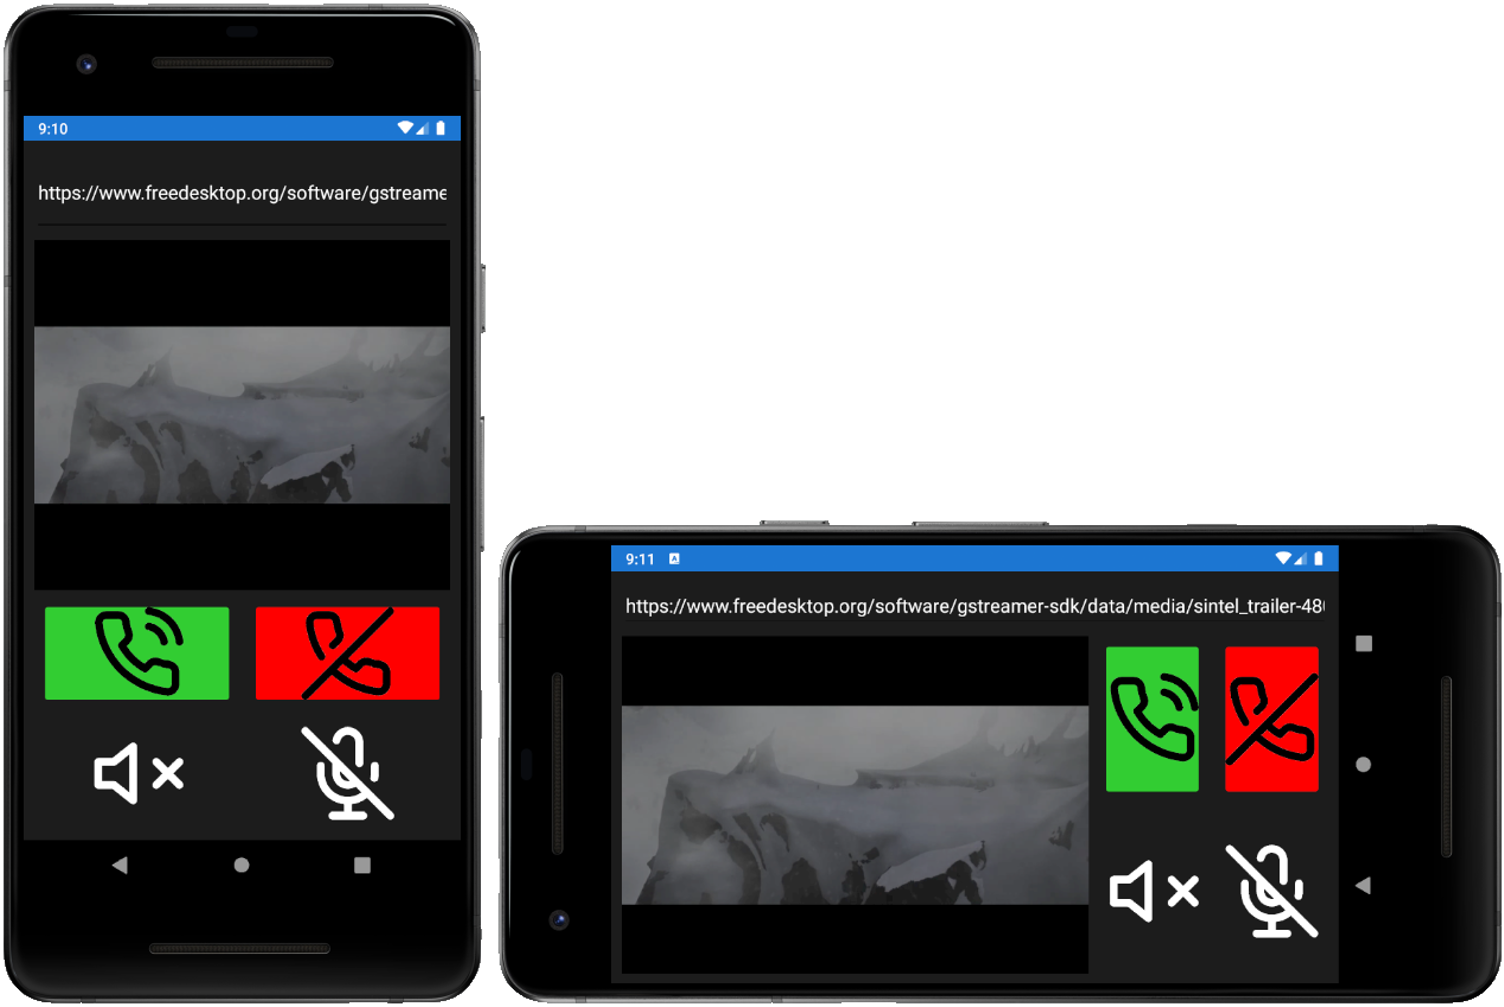
\includegraphics[width=.9\linewidth]{images/projektergebnis/ansichtenFinaleApp.png}
    \caption{App-Ansichten}
\end{figure}

Aus diesen Software-Teilen wurde eine fertige Android-Applikation erstellt, mit der der Fernzugriff auf die fest installierte Videosprechanlage jederzeit möglich ist.
Die Kommunikation wurde bidirektional für die Ton- und unidirektional für die Video-Übertragung realisiert.
Die Applikation wurde auf verschiedenen Systemen simuliert und in geringem Ausmaß getestet.
Eine iOS-Version wurde aufgrund fehlender Endgeräte nicht fertiggestellt bzw. getestet.\par

Die programmierte Applikation ist in diesem Dokument ausführlich beschrieben und wesentliche Funktionen im Detail erklärt.
Die Erläuterung des Programm-Codes ist kein normrelevantes Regelwerk, sondern ein Kommentar wie es der Autor \AndreasGrain\ versteht!
Im Zweifelsfall wird darauf hingewiesen, dass die offiziellen Angaben der Hersteller zu verwenden sind.
Auf diese wird an relevanten Stellen verwiesen.

Verwendete Technologien und Software:
\begin{itemize}
    \item RTSP zur Übertragung der Mediendaten über das Netzwerk
    \item LibVLC Sharp zum Abrufen und Darstellen des Video-Streams
    \item GStreamer zur Weiterverarbeitung der Mediendaten am Server
    \item Live555 Proxy zum Verteilen des RTSP-Streams
    \item Push Benachrichtigung zur Kontaktaufnahme mit dem Benutzer der App
    \item Visual Studio 2019 als Entwicklungsumgebung
    \item Xamarin-Rahmenwerk für die Entwicklung der Multiplattform-App
    \item \hologo{XeLaTeX} zur Erstellung der Dokumentation
    \item OneNote zur Projektplanung
\end{itemize}